%!TEX root = ../../../main.tex



	% \subsection{Sideband} \label{subsubsec::sideband}
	%
	% 	\todo{beginning new}As mentioned before, phonons of the diamond lattice and the color center manifenst themselves as peaks in the sideband of the \pl spectrum.
	% 	Phonons reduce the intensity of the the purely electronic transition, the \zpl.
	% 	The electron-phonon coupling is quantified by the \db factor or the \hr.
	% 	The former is the integrated intensity of the \zpl $I_{ZPL}$ divided by the integrated intensity of the \pl of the whole spectrum, i.e. \ZPL plus sidebands, $I_{tot}$ \cite{Neu2014,Gaebel2004}.
	% 	The \hr factor $S$ is defined as $I_{ZPL}/I_{tot}=\exp{-S}$.\todo{end new}
	%
	%
	% 	\begin{figure}[tp]
	% 		\centering
	% 		\testbox{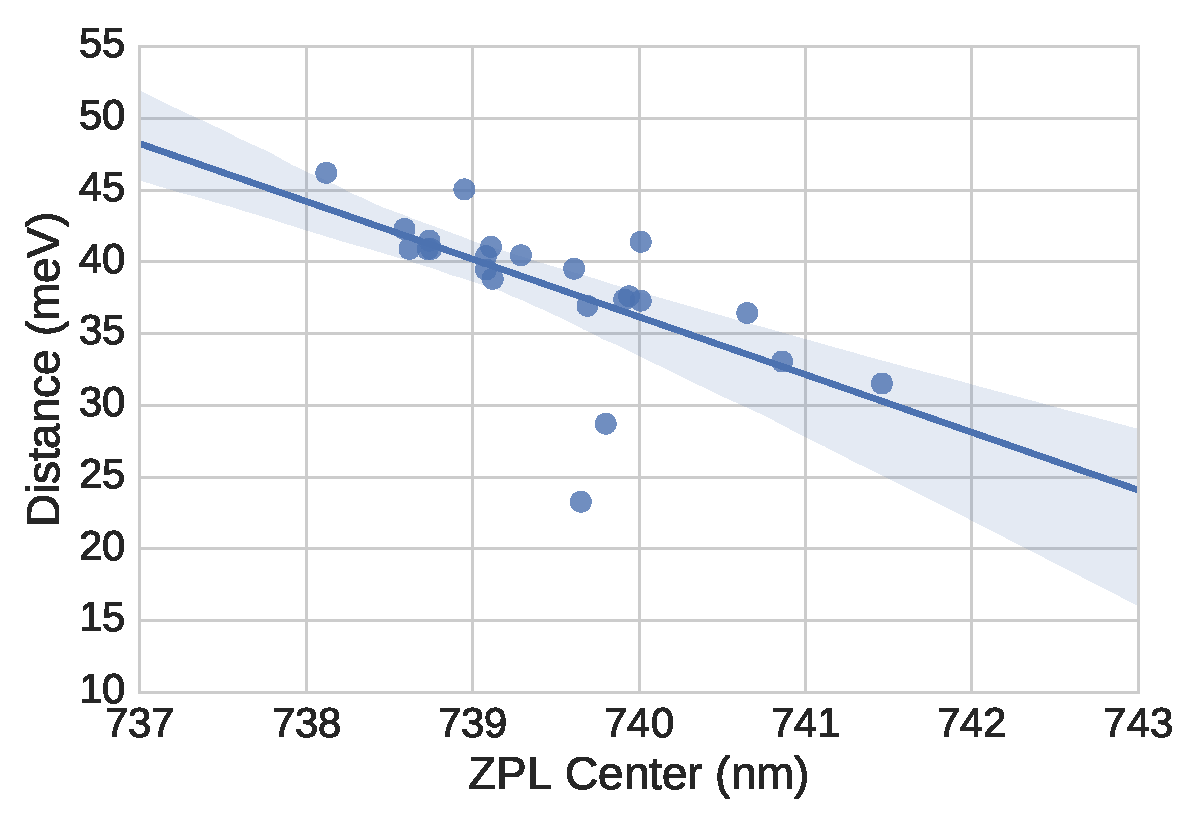
\includegraphics[trim = 0 0 0 0,  clip= true, width = 0.49\textwidth]{./pics/sideband_regression.pdf}}
	% 		\caption{Shift of dominant sideband peak from the \ZPL in spectra of \sivs (\vl, samples \insituF, \insituS, \insituH) vs. ZPL \cwl. The linear fit shows that the shift decreases with increasing ZPL center wavelength. The shaded area is the 95\% confidence interval.}
	% 		\label{fig::sideband_fit}
	% 	\end{figure}
	%
	% 	\begin{figure}[tp]
	% 		\centering
	% 		\testbox{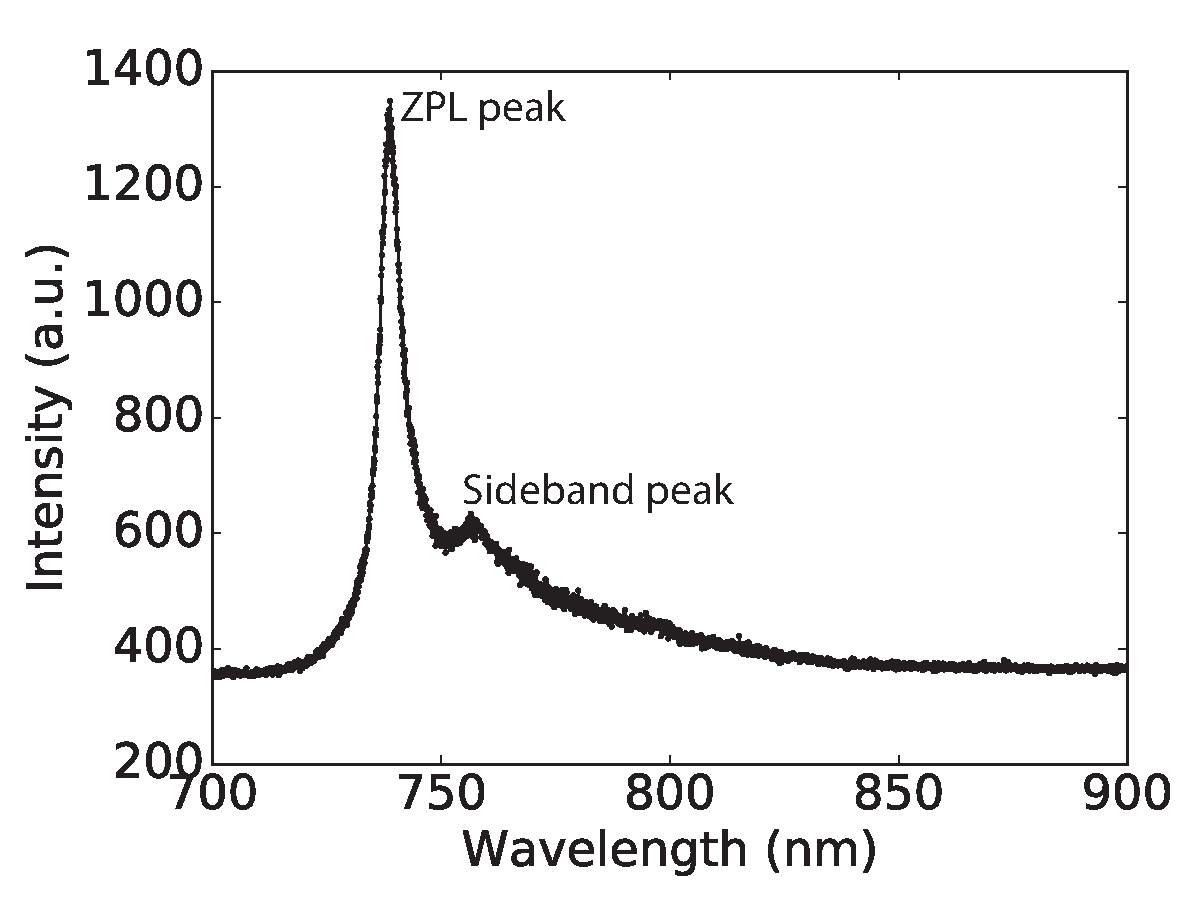
\includegraphics[trim = 0 0 0 0,  clip = true, width = 0.49\textwidth]{./pics/Ir25M_spe_scan_xy-38x9y16_300uW_t120.pdf}}
	% 		\caption{Representative spectrum of an emitter of \vl exhibiting a sideband peak.}
	% 		\label{fig::broad_peak_sb}
	% 	\end{figure}
	%
	% 	From literature it is known, that the \siv in \nd exhibits a large \db of over 70\% \cite{Neu2011,Neu2011b}, which is consistent with our measurements of \emnarrow and \embroad.
	% 	Nevertheless, sideband peaks are present in many \siv PL emission spectra.
	% 	The investigated emitters exhibit two different structures of sideband spectra: The spectra in \vl exhibit one strong sideband peak (\autoref{fig::broad_peak_sb}), spectra in \hl exhibit several weaker sideband peaks.
	% 	\\
	% 	However, there is no recurring pattern in the sideband of \hl.
	% 	The challenge arises to unequivocally distinguish between peaks stemming from a phonon sideband and peaks stemming from shifted, less intense \siv \ZPLs.
	% 	The possibility exists, that some peaks identified as phonon sidebands are actually ZPLs stemming from shifted \sivs.
	% 	Therefore, we will focus our investigations on the more prominent sideband of \vl.
	% 	\\
	% 	Most of the spectra in \vl exhibit a characteristic shape, composed of the ZPL and one strong sideband peak which is mostly shifted \SIrange{37}{43}{meV}.
	% 	In reference \cite{Dietrich2014} the \SI{42}{meV} sideband peak is attributed to a non-localized (lattice) mode.
	% 	It is also stated, that the local vibrational mode at \SI{64}{meV} is much stronger than the  \SI{42}{meV} sideband peak.
	% 	While the peak attributed to the non-localized mode is very strong in our measurements, we cannot identify the peak attributed to the local vibrational \siv mode in the spectra of \vl.
	% 	A possible explanation is, that the lattice mode at \SIrange{37}{43}{meV} is so strong that the local vibrational mode at \SI{64}{meV} cannot be separated from the tail of the lattice mode.
	% 	In \autoref{fig::sideband_fit} the distance between the \cwl of the sideband peak and the \cwl of the ZPL is plotted against the ZPL \cwl.
	% 	The distribution is fitted with a linear regression.
	% 	We attribute the variance in the sideband shift to strain: \correct{Adam Galis Erkenntnisse}
	% 	\\
	% 	\todo{beginning new}For further investigations, we plotted the \ZPL  of \vl with multiple peaks.
	% 	We found that two Lorentzian fits fit the peak best.
	% 	\autoref{fig::sideband_multfit} shows histograms of the distribution of the \cw and the \lw of the fitted peaks.
	% 	Keep in mind that two of the peaks sum up to the peak visible as a \ZPL and the third peak is the sideband peak which we attribute to a lattice mode.
	% 	We found that the \lw of the sideband peak exhibits values up to \SI{20}{nm}.
	% 	This broad width is an indicator, that the local vibrational mode might indeed be outpowered by the more intense lattice mode.
	% 	However, it is not very easy to find spectra where the sideband peak is pronounced and isolated enough to make proper statistics.
	% 	The original \ZPL is split up in two peaks, one with a median \cwl of \SI{738}{nm} and a median \lw of \SI{4.5}{nm} and the other with a median \cwl of \SI{742}{nm} and a median \lw of \SI{8}{nm}.\todo{correct and verify all numbers}
	% 	It could be that this is an indication for another sideband peak at \SI{742}{nm}.
	% 	This assumption could be verified by cryostatic measurements, where the phonon sideband should vanish and only the \ZPL survive and split up into the four-level fine structure.
	% 	\todo{end new}
	% 	\\
	% 	\begin{figure}[tp]
	% 		\begin{subfigure}[t]{ 0.49\linewidth}
	% 			\centering
	% 			\caption{}
	% 			\testbox{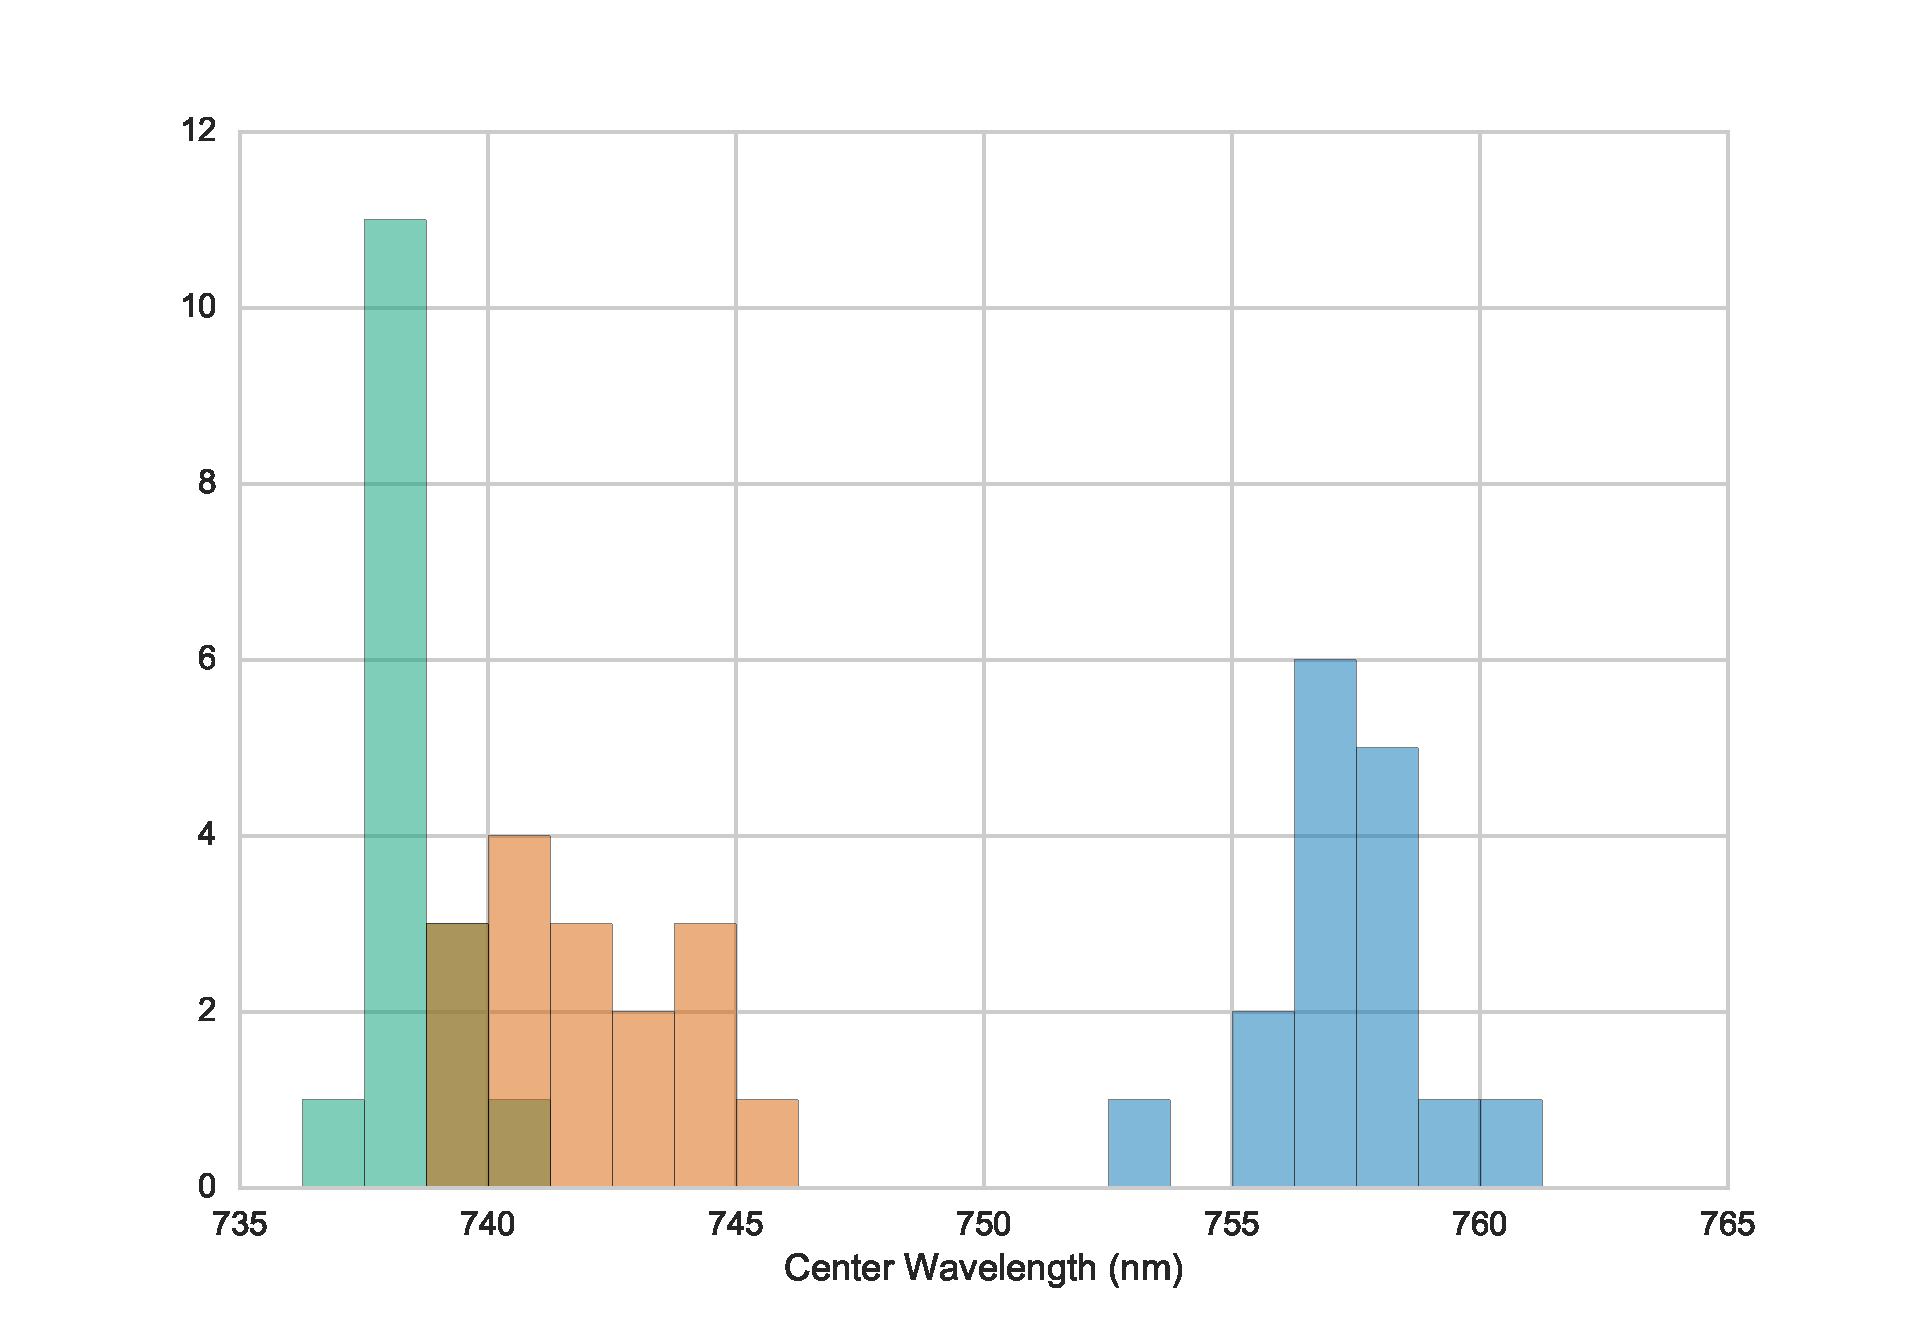
\includegraphics[trim = 0 0 0 0,  clip= true, width = \textwidth]{./pics/histo_multi_sidebands_position25bins.pdf}}
	% 			\label{subfig::sb_multfit_pos}
	% 		\end{subfigure}
	% 		\hfill
	% 		\begin{subfigure}[t]{ 0.49\linewidth}
	% 			\centering
	% 			\caption{}
	% 			\testbox{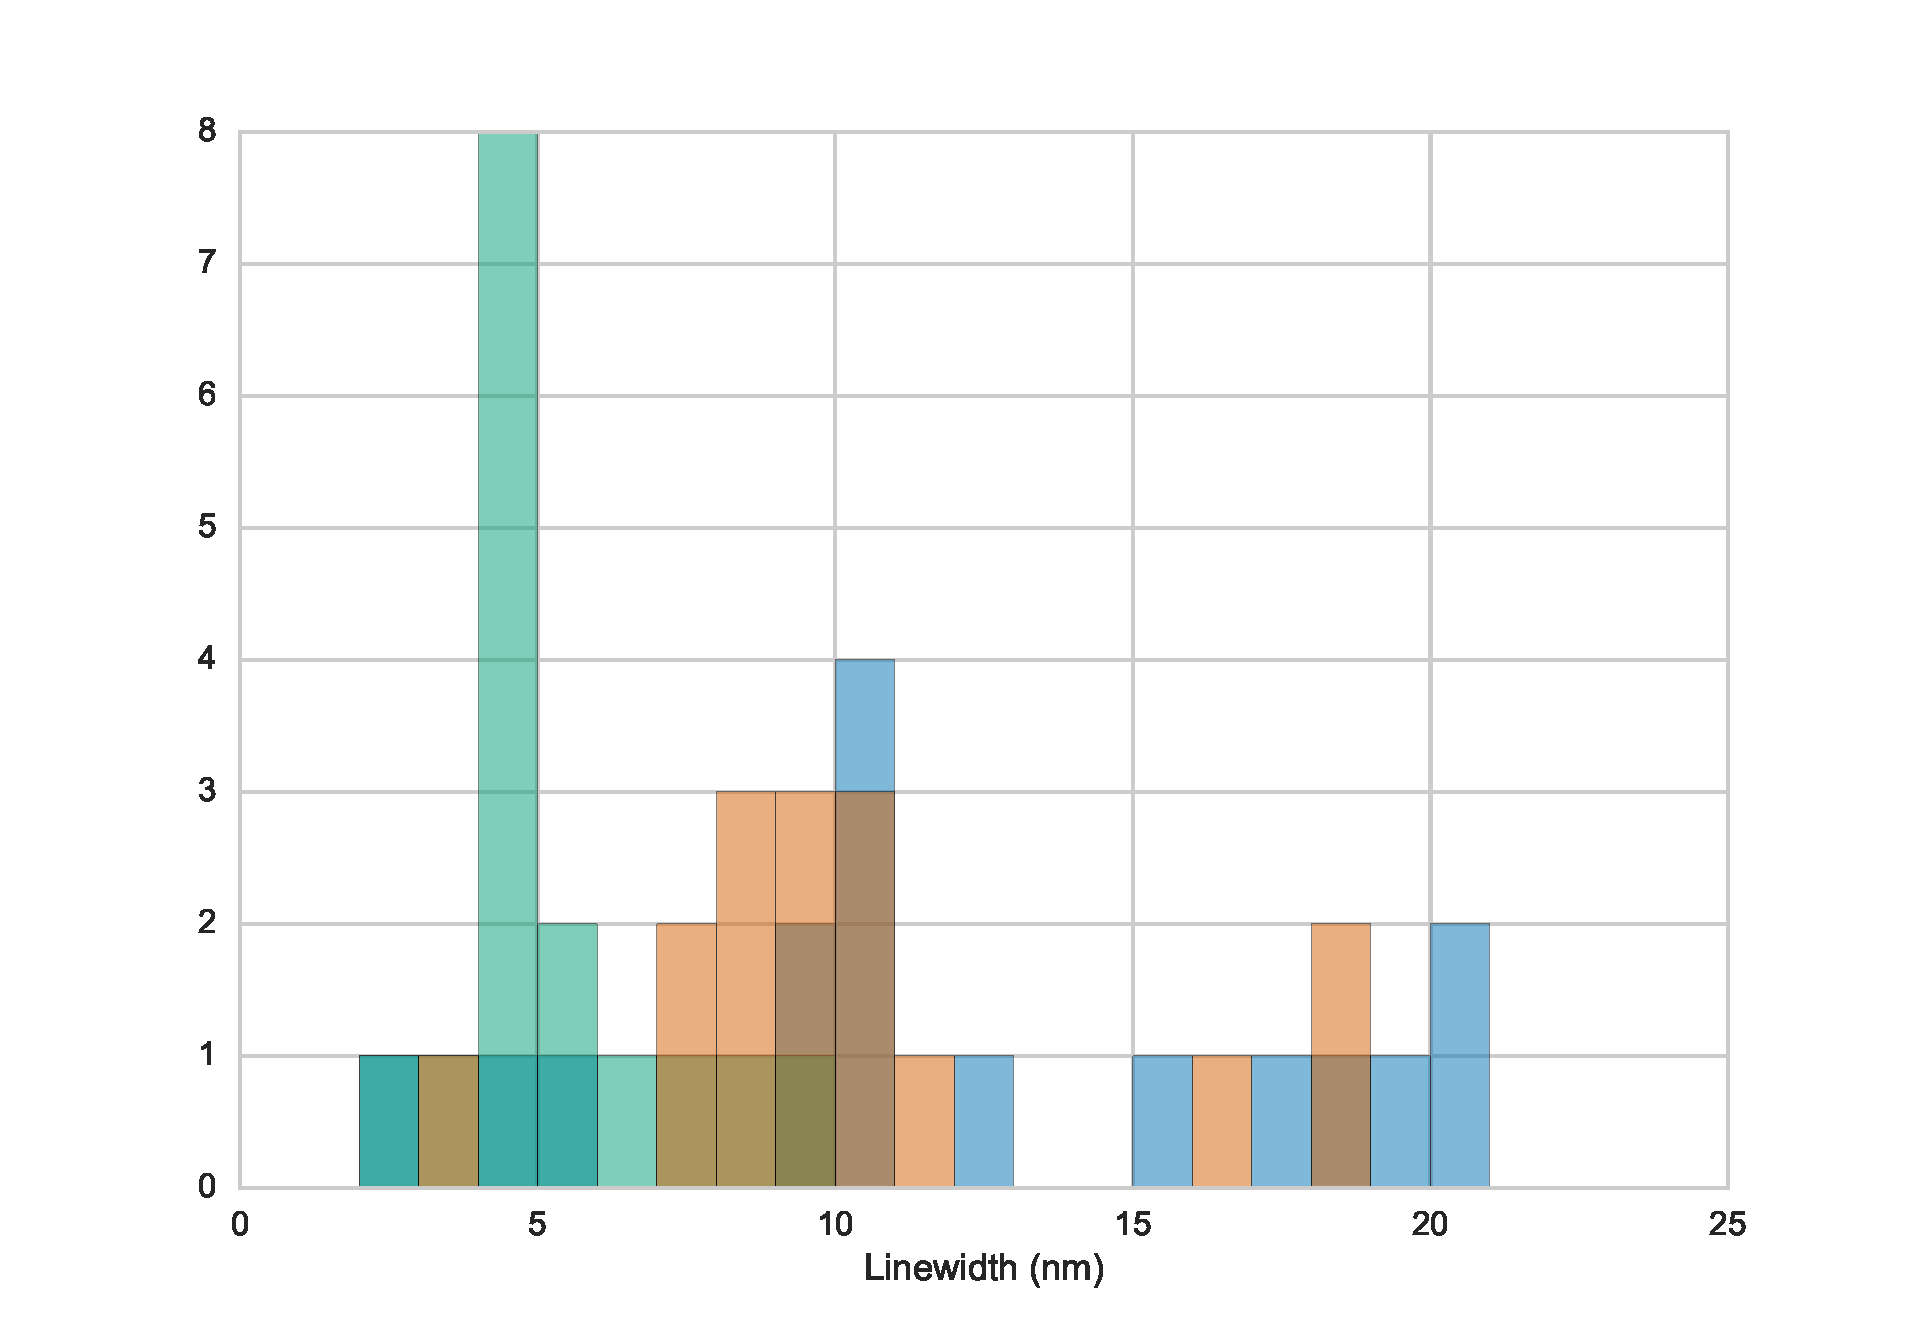
\includegraphics[trim = 0 0 0 0,  clip= true, width = \textwidth]{./pics/histo_multi_sidebands_width_25bins.pdf}}
	% 			\label{subfig::sb_multfit_width}
	% 		\end{subfigure}
	% 		\caption{}
	% 		\label{fig::sideband_multfit}
	% 	\end{figure}
	%
	%
	% \subsection{Cryostatic Measurements}\label{subsec::cryo}
	%
	% 	\begin{figure}[tp]
	% 		\begin{subfigure}[t]{ 0.49\linewidth}
	% 			\centering
	% 			\caption{}
	% 			\testbox{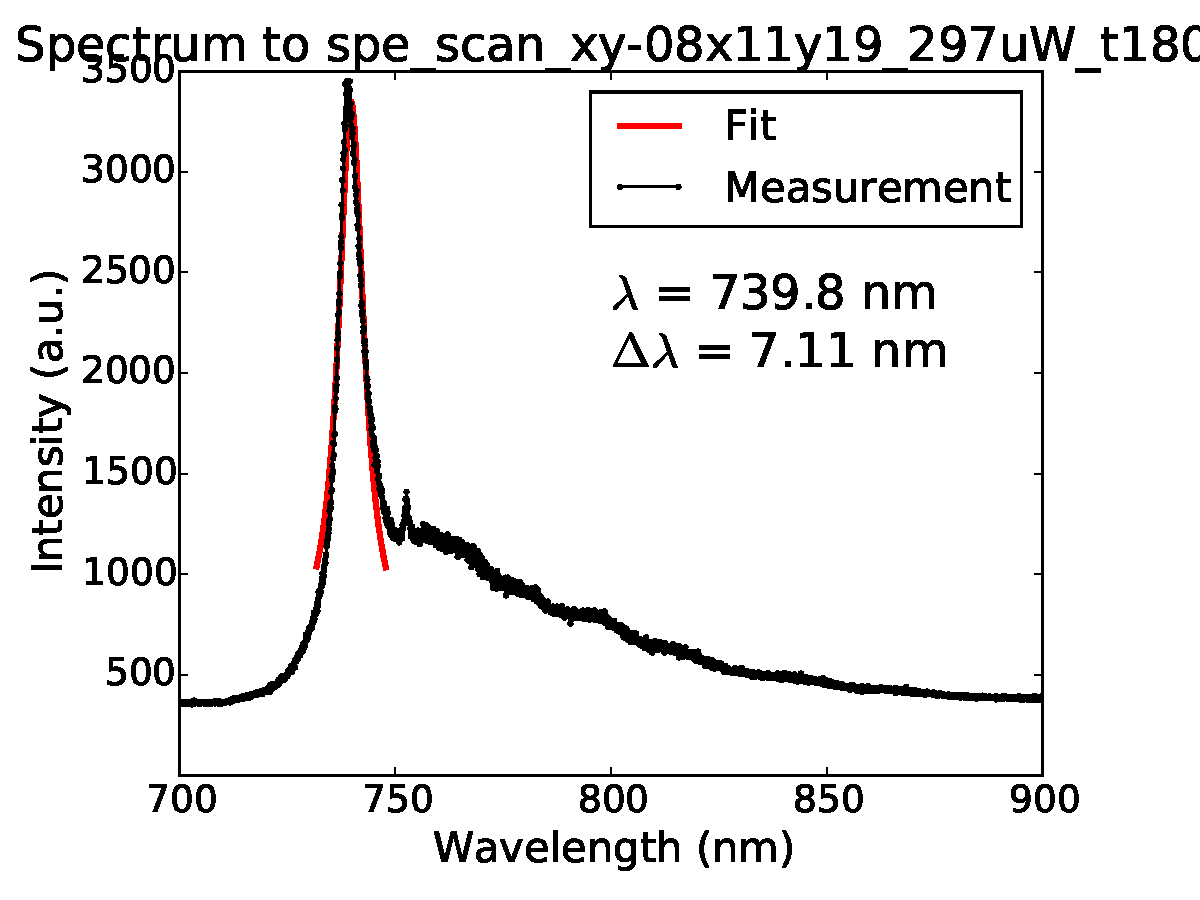
\includegraphics[trim = 0 0 0 0,  clip= true, width = \textwidth]{./pics/Ir25Mox_fit_spe_scan_xy-08x11y19_297uW_t180.pdf}}
	% 			\label{subfig::roomtep1}
	% 		\end{subfigure}
	% 		\hfill
	% 		\begin{subfigure}[t]{ 0.49\linewidth}
	% 			\centering
	% 			\caption{}
	% 			\testbox{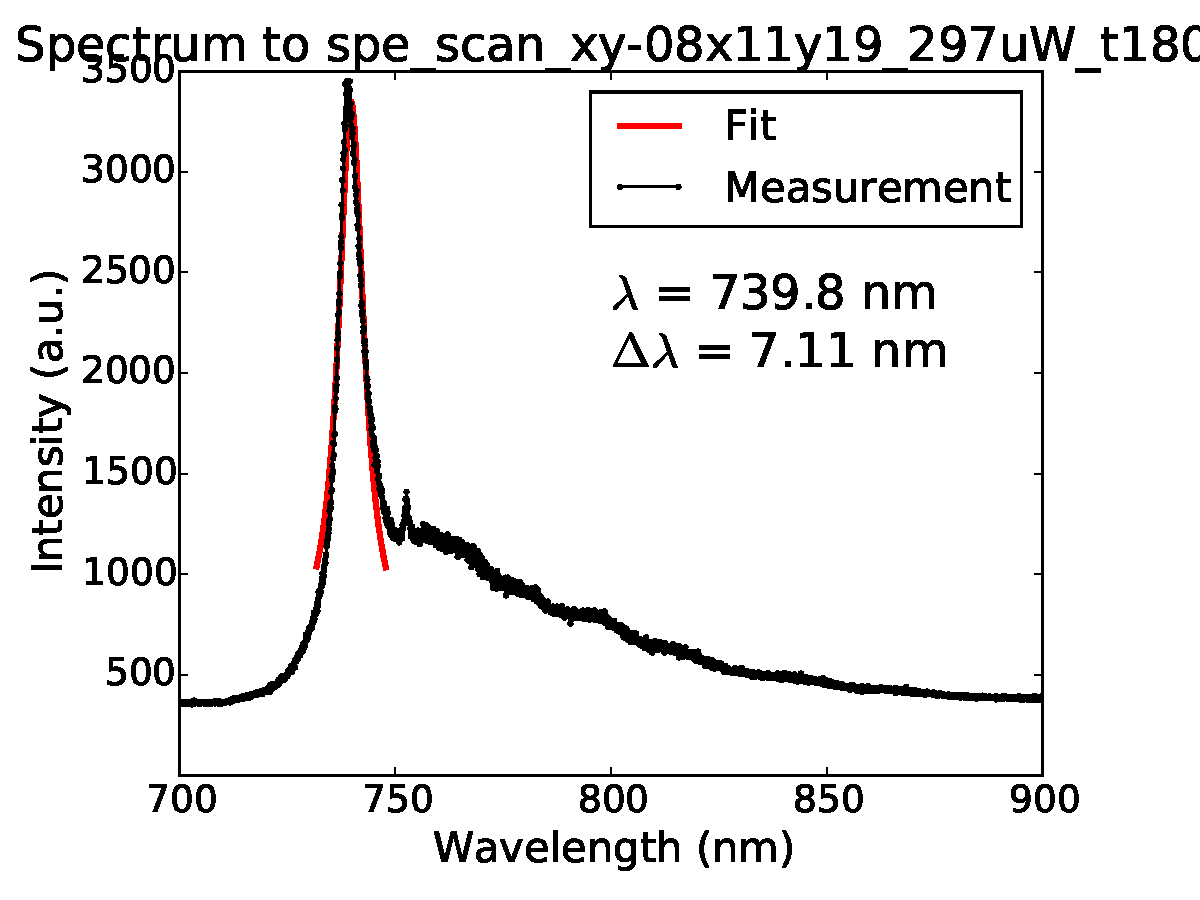
\includegraphics[trim = 0 0 0 0,  clip= true, width = \textwidth]{./pics/Ir25Mox_fit_spe_scan_xy-08x11y19_297uW_t180.pdf}}
	% 			\label{subfig::cryo}
	% 		\end{subfigure}
	% 		\caption{}
	% 		\label{fig::rt_vs_cryo1}
	% 	\end{figure}
	%
	% 	\begin{figure}[tp]
	% 		\begin{subfigure}[t]{ 0.49\linewidth}
	% 			\centering
	% 			\caption{}
	% 			\testbox{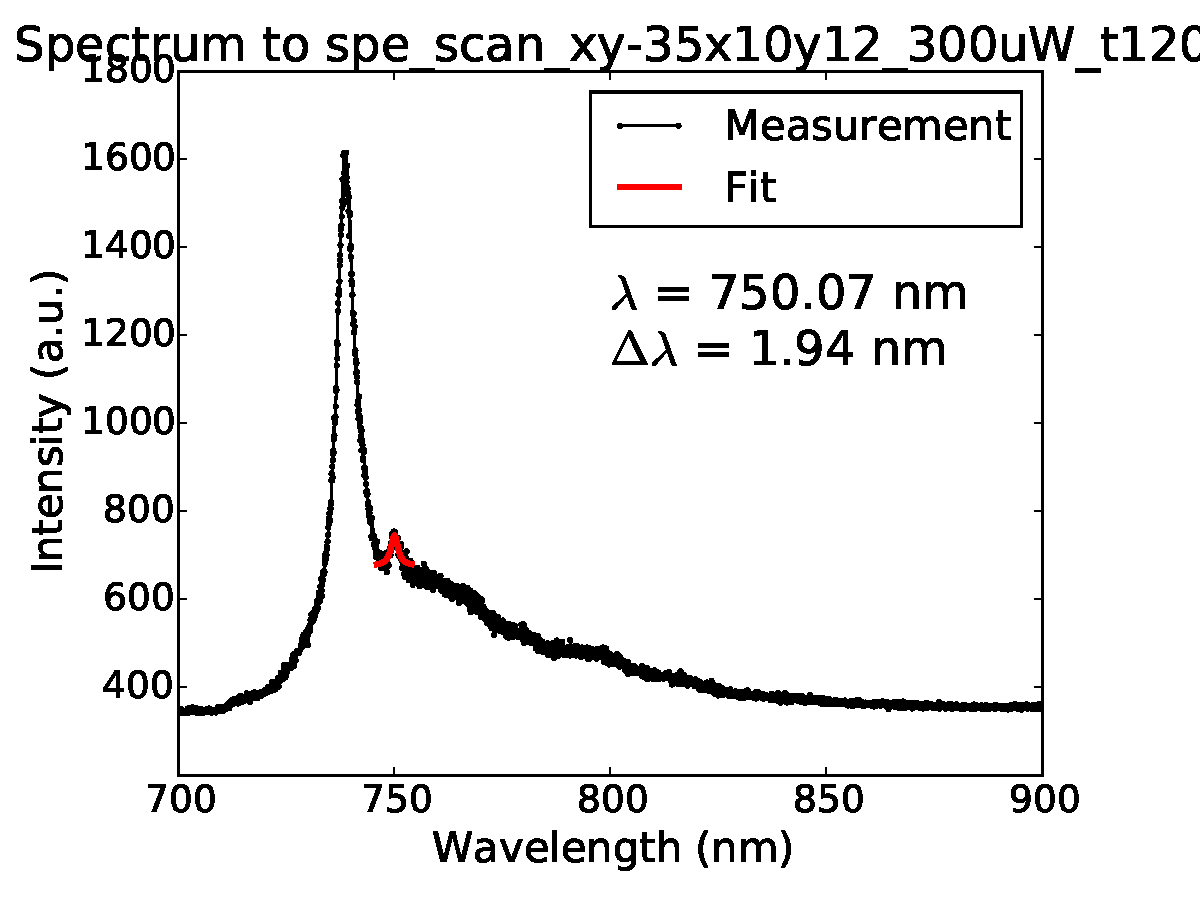
\includegraphics[trim = 0 0 0 0,  clip= true, width = \textwidth]{./pics/Ir25Mox_spe_scan_xy-35x10y12_300uW_t120_fit.pdf}}
	% 			\label{subfig::roomtep2}
	% 		\end{subfigure}
	% 		\hfill
	% 		\begin{subfigure}[t]{ 0.49\linewidth}
	% 			\centering
	% 			\caption{}
	% 			\testbox{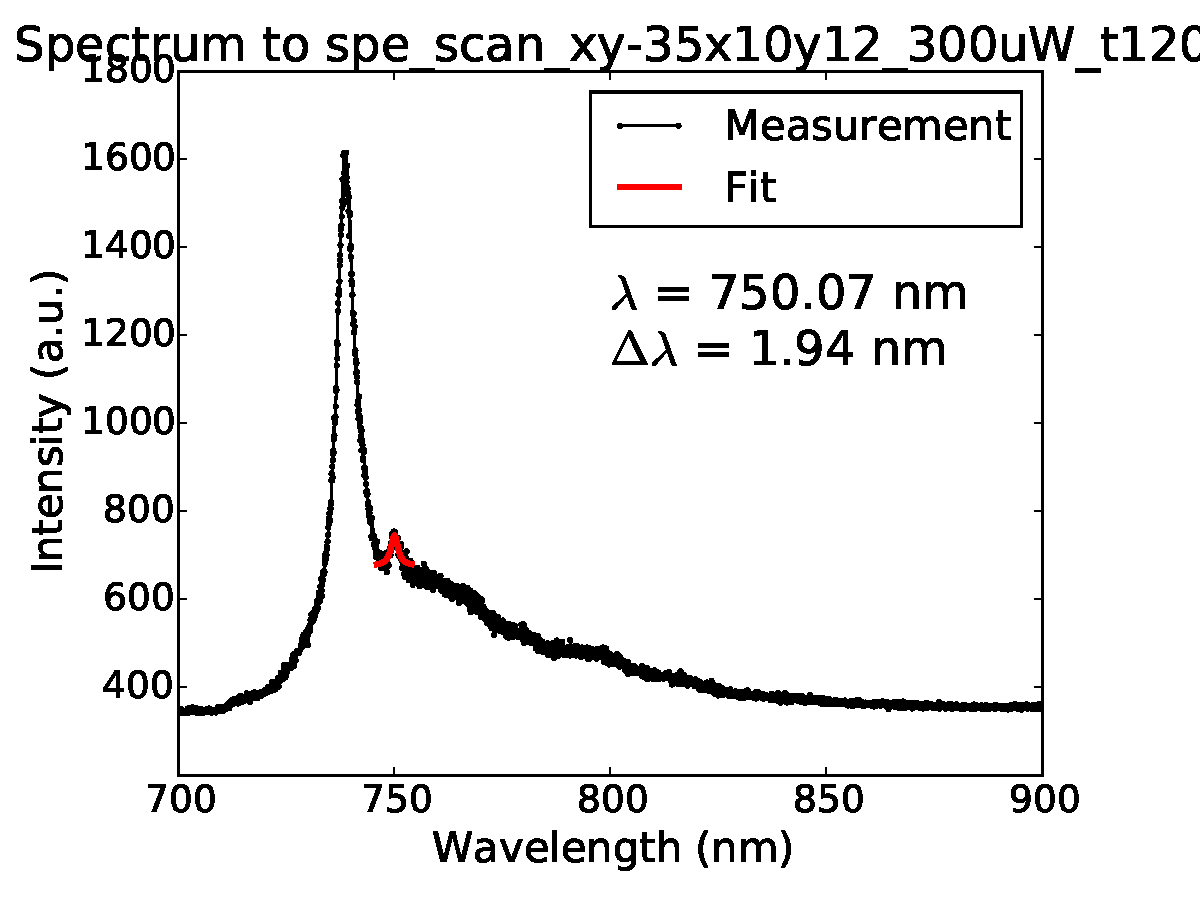
\includegraphics[trim = 0 0 0 0,  clip= true, width = \textwidth]{./pics/Ir25Mox_spe_scan_xy-35x10y12_300uW_t120_fit.pdf}}
	% 			\label{subfig::cryo2}
	% 		\end{subfigure}
	% 		\caption{}
	% 		\label{fig::rt_vs_cryo2}
	% 	\end{figure}
	%
	% 	We performed some cryostatic measurements to to pursue two goals:
	% 	First, if we see the four-level splitting of the \ZPL this is further proof that the dominant peaks of our spectra are indeed all due to \sivs and do not stem from other impurities.
	% 	Second, if the sideband peaks vanish at cold temperatures, this is evidence that they are caused by phonons.
	% 	So we cooled down a sample, but all we saw was a wood of lines.
	% 	Apparently, there were multiple \sivs in the \nds and they were all strained, messing up the four-level line structure.


	\subsection{Sideband} \label{subsubsec::sideband}

		It is known that the \pl spectra of \sivs in \nd are dominated by the \zpl. As a result \psb contributions remain small, a fact expressed in large \db factors of over \SI{70}{\percent} established previously \cite{Neu2011,Neu2011b}. Our own measurements are consistent with these of \emnarrow and \embroad results. We also find distinct sideband peaks in many \siv \pl emission spectra.
		The investigated emitters exhibit two different structures of sideband spectra: The spectra in \vl exhibit one strong sideband peak, spectra in \hl exhibit several weaker sideband peaks. \autoref{subfig::sideband_group_v} and \autoref{subfig::sideband_group_h} illustrate the respective observations.

		\begin{figure}[htp]
			\begin{subfigure}[t]{ 0.49\linewidth}
				\centering
				\caption{}
				\testbox{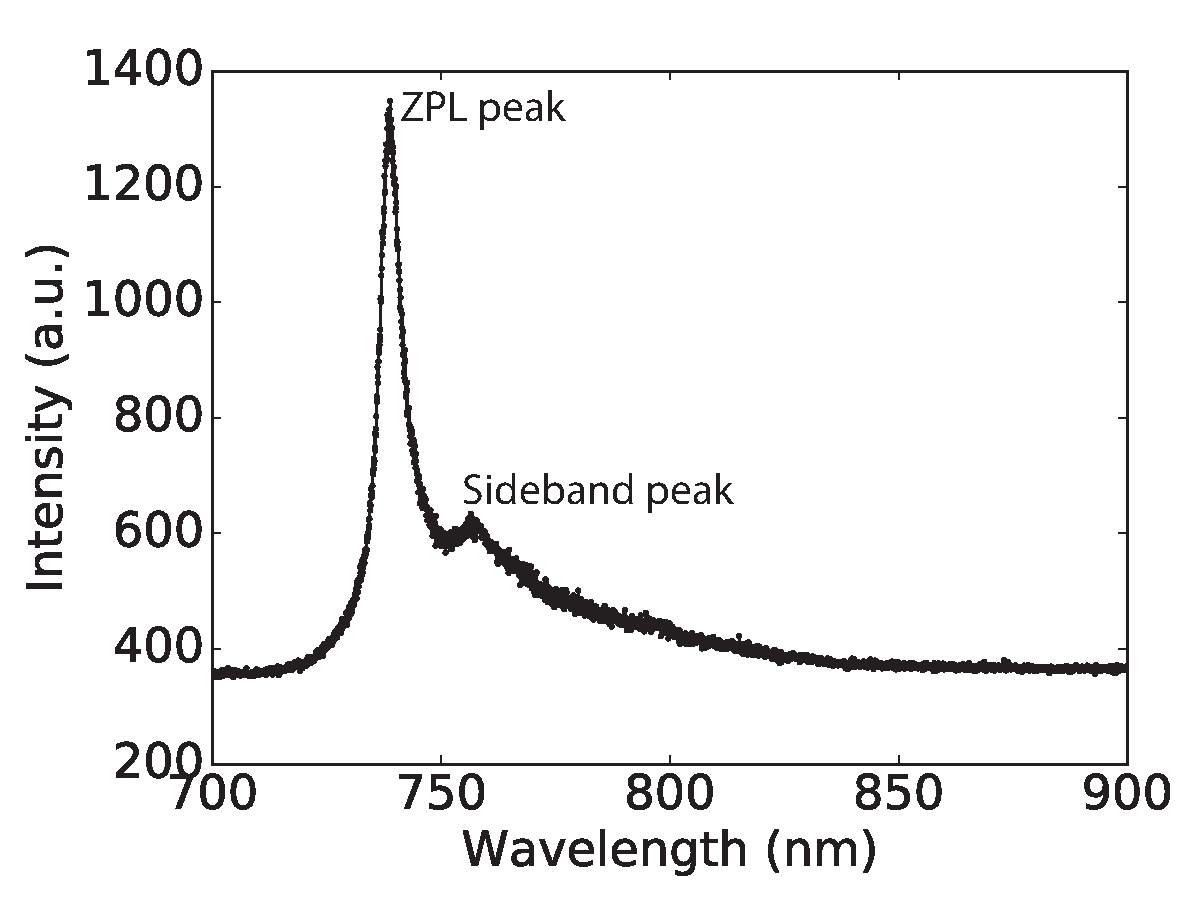
\includegraphics[trim = 0 0 0 0,  clip= true, width = \textwidth]{./pics/Ir25M_spe_scan_xy-38x9y16_300uW_t120.pdf}}
				\label{subfig::sideband_group_v}
			\end{subfigure}
			\hfill
			\begin{subfigure}[t]{ 0.49\linewidth}
				\centering
				\caption{}
				\testbox{\includegraphics[trim = 0 0 0 0,  clip= true, width = \textwidth,draft]{./pics/<weaker sidebands here>.pdf}}
				\label{subfig::sideband_group_h}
			\end{subfigure}
			\caption[Side band peaks for \sivs]{Representative spectra of emitters showing single (\subref{subfig::sideband_group_v}) and multiple (\subref{subfig::sideband_group_h}) side band peaks. The former belong to \vl, while the latter are members of \hl.}
			\label{fig::sideband_groups}
		\end{figure}

		Most of the spectra in \vl exhibit a characteristic shape, composed of the \ZPL and one strong sideband peak.
		\SI{70}{\percent} of the \pl spectra with one distinct sideband peak exhibit a shift of the sideband peak from the \ZPL between \SIrange{37}{43}{meV}.
		The range of line shifts for the prominent sideband peak coincides with a well-known feature at \SI{42}{meV}, associated with \sivs \cite{Larkins1971,Sternschulte1994}, but also to a larger number of optically active defects \cite{Sternschulte1994}.
		The occurrence of this \SI{42}{meV} sideband feature for a large number of defects and the absence of isotopic variations \cite{Dietrich2014}, favors an assignment as non-localized lattice vibration.
		We furthermore observe that the dominant sideband peak shifts towards smaller distance from the \ZPL for increasing \ZPL \cwl, i.e.\ increasing strain. \autoref{fig::sideband_fit} presents a linear fit to data for emitters in \vl..
		The low phonon energy of the sideband feature and its shift with strain might arise from a local ``softening'' of the crystal lattice in the vicinity of a defect \cite{Sternschulte1994}.

		\begin{figure}[htp]
			\centering
			\testbox{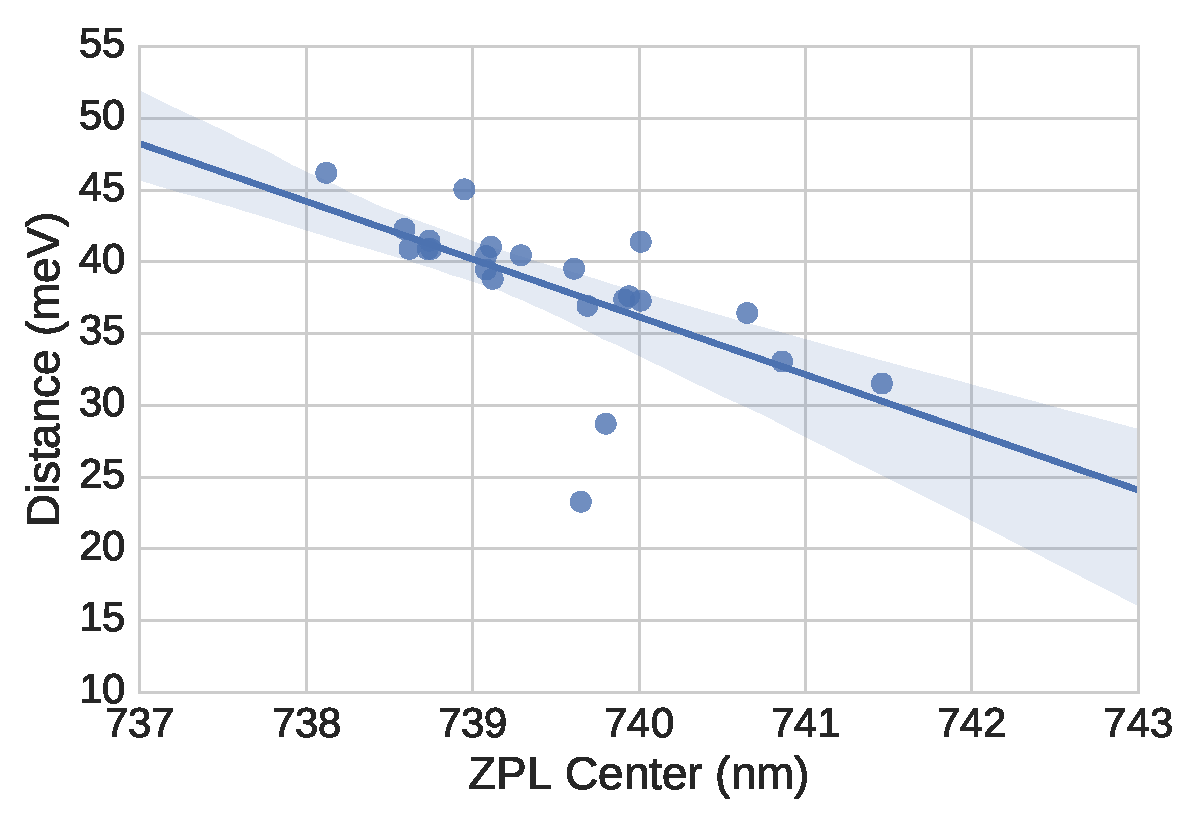
\includegraphics[trim = 0 0 0 0,  clip= true, width = 0.49\textwidth]{./pics/sideband_regression.pdf}}
			\caption[Shift of dominant side band peaks for \sivs]{Shift of dominant sideband peak from the \ZPL in spectra of \sivs (\vl, samples \insituF, \insituS, \insituH) vs. ZPL \cwl. The linear fit shows that the shift decreases with increasing ZPL center wavelength, i.e.\ with increasing strain and exhibits a slope of \SI[separate-uncertainty]{-4\pm1}{\milli\electronvolt\per\nano\meter}. The shaded area is the \SI{95}{\percent} confidence region.}
			\label{fig::sideband_fit}
		\end{figure}

		A recent study \cite{Londero2016} suggests that the \SI{42}{meV} mode, similar to other broad \psb features, originates from a resonance attributed to phonons causing the dynamical Jahn-Teller effect with \sivs \cite{Fu2009}.
		As the Jahn-Teller coupling varies with strain it is also expected that the resonance shifts accordingly.
		\\
		In the spectra of \vl, we do not observe a typical \siv sideband feature at \SI{64}{meV}, attributed to a local vibration of the \si atom, frequently much stronger than the  \SI{42}{meV} sideband peak.
		A possible explanation is, that the lattice mode at \SIrange{37}{43}{meV} is so strong that the local vibrational mode at \SI{64}{meV} cannot be separated from the tail of the lattice mode.
		\\
		In \hl we observe many spectra which exhibit several peaks within the spectral range of our detection range between \SIrange{710}{900}{nm}.
		The challenge arises to unequivocally distinguish between peaks stemming from a phonon sideband and peaks stemming from shifted, less intense \siv \ZPLs.

		Interestingly, we assert a tendency for peaks to accumulate at a shift of around \SIlist{43;64;150;175}{meV}. This pattern in the \psb of \hl is consistent with side band shifts reported in \cite{Sternschulte1994,Zaitsev2000, Neu2011}.

		The possibility exists, that some these peaks believed to be \psbs are actually shifted \ZPLs stemming from other \sivs. To address this question, we perform \pl measurements at cryogenic temperatures.


		\subsection{Cryostatic Measurements}\label{subsec::cryo}

			\begin{figure}[htp]
				\begin{subfigure}[t]{ 0.49\linewidth}
					\centering
					\caption{}
					\testbox{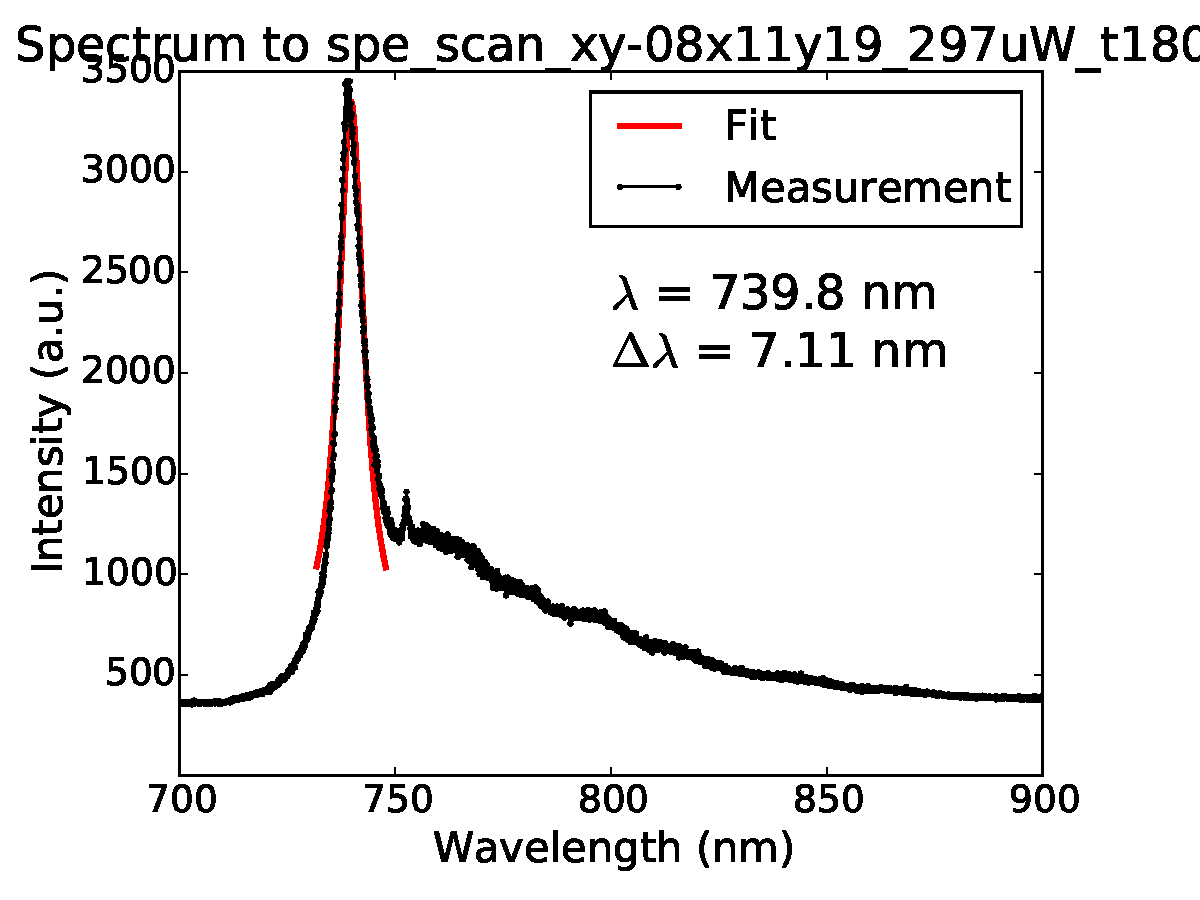
\includegraphics[trim = 0 0 0 0,  clip= true, width = \textwidth]{./pics/Ir25Mox_fit_spe_scan_xy-08x11y19_297uW_t180.pdf}}
					\label{subfig::roomtep1}
				\end{subfigure}
				\hfill
				\begin{subfigure}[t]{ 0.49\linewidth}
					\centering
					\caption{}
					\testbox{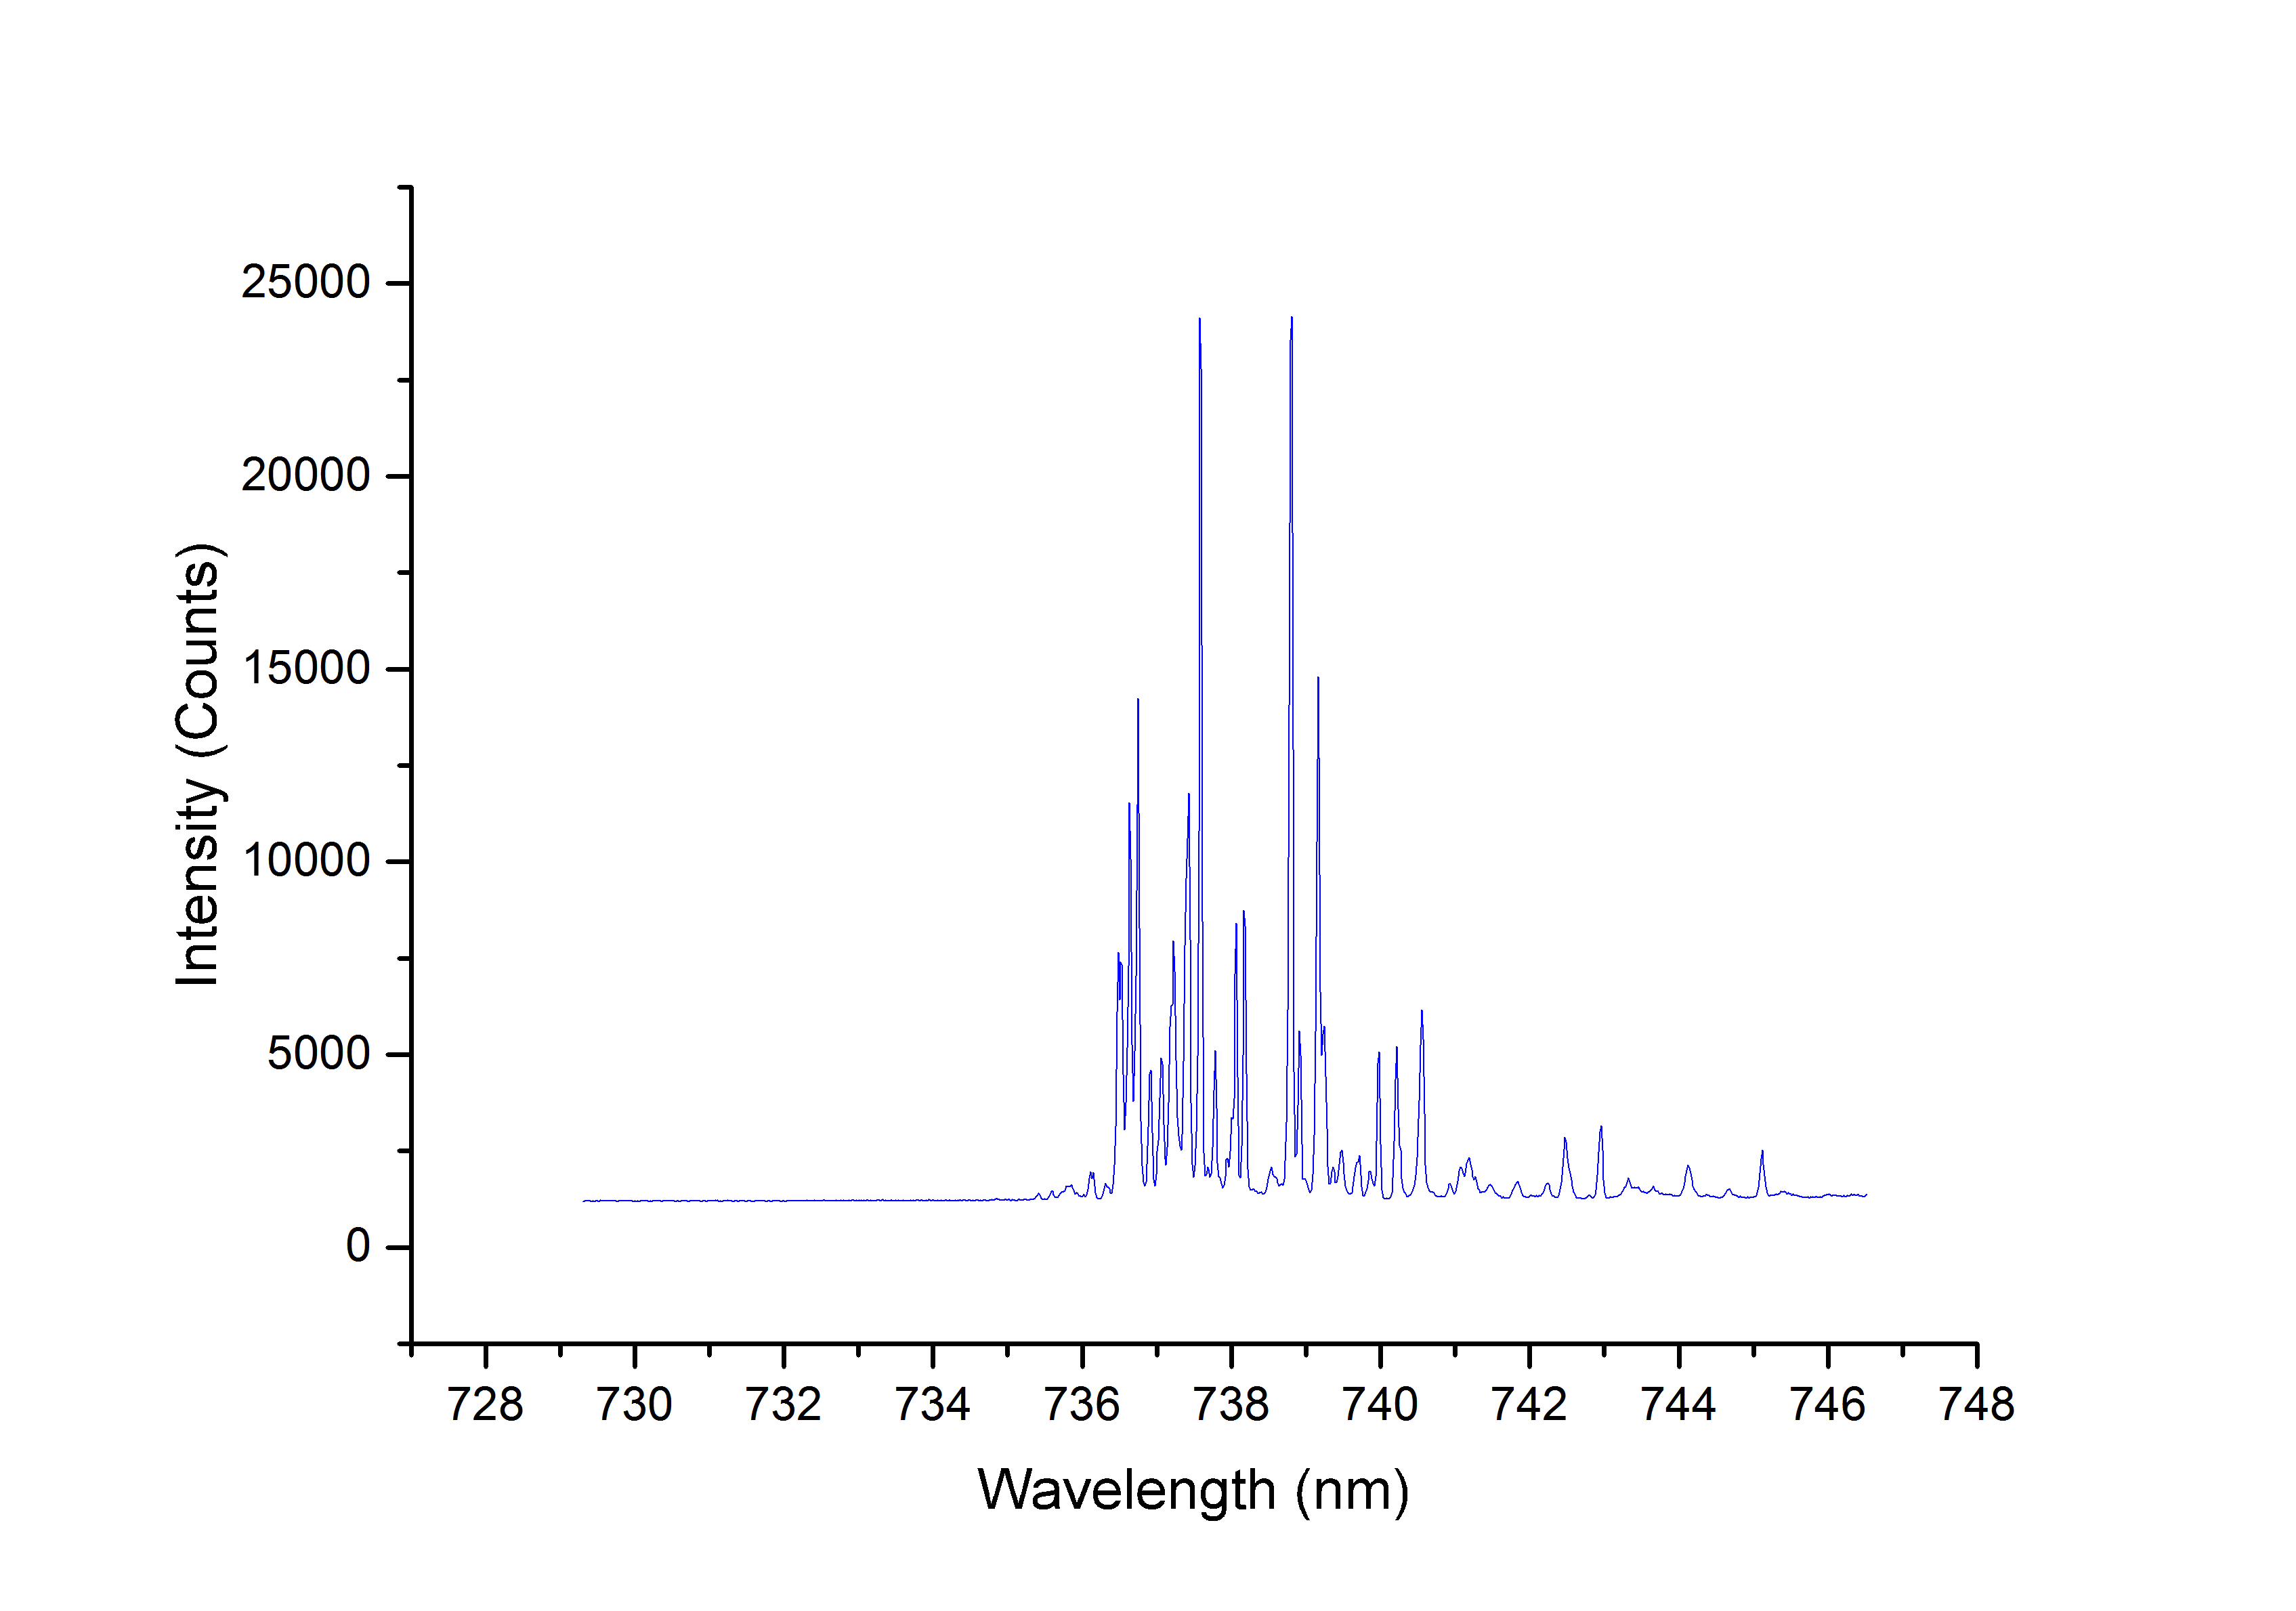
\includegraphics[trim = 0 0 0 0,  clip= true, width = \textwidth]{./pics/cryo_Spektrum68_edit.png}}
					\label{subfig::cryo1}
				\end{subfigure}
				\hfill
				\begin{subfigure}[t]{ 0.49\linewidth}
					\centering
					\caption{}
					\testbox{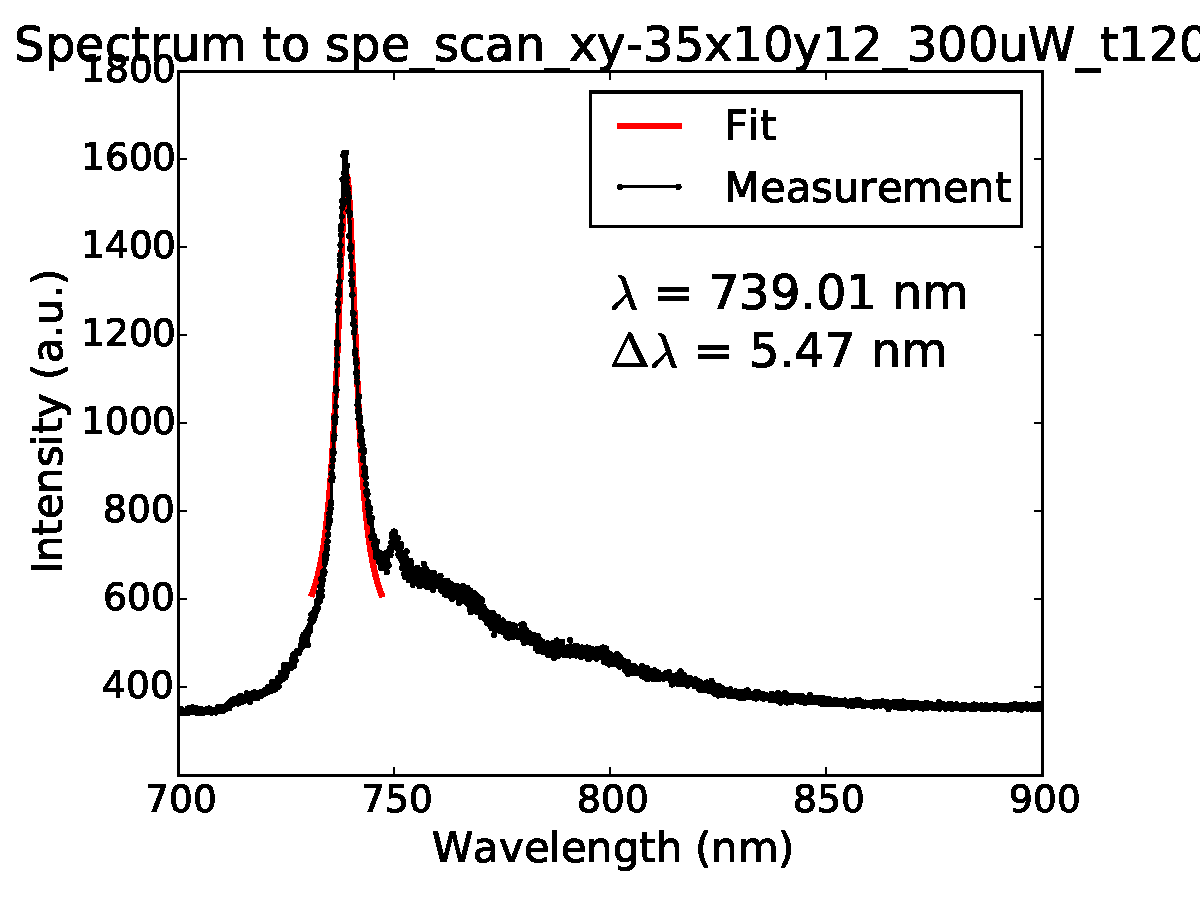
\includegraphics[trim = 0 0 0 0,  clip= true, width = \textwidth]{./pics/Ir25M_rt_to_cryo_84_fit_spe_scan_xy-35x10y12_300uW_t120.pdf}}
					\label{subfig::roomtep2}
				\end{subfigure}
				\hfill
				\begin{subfigure}[t]{ 0.49\linewidth}
					\centering
					\caption{}
					\testbox{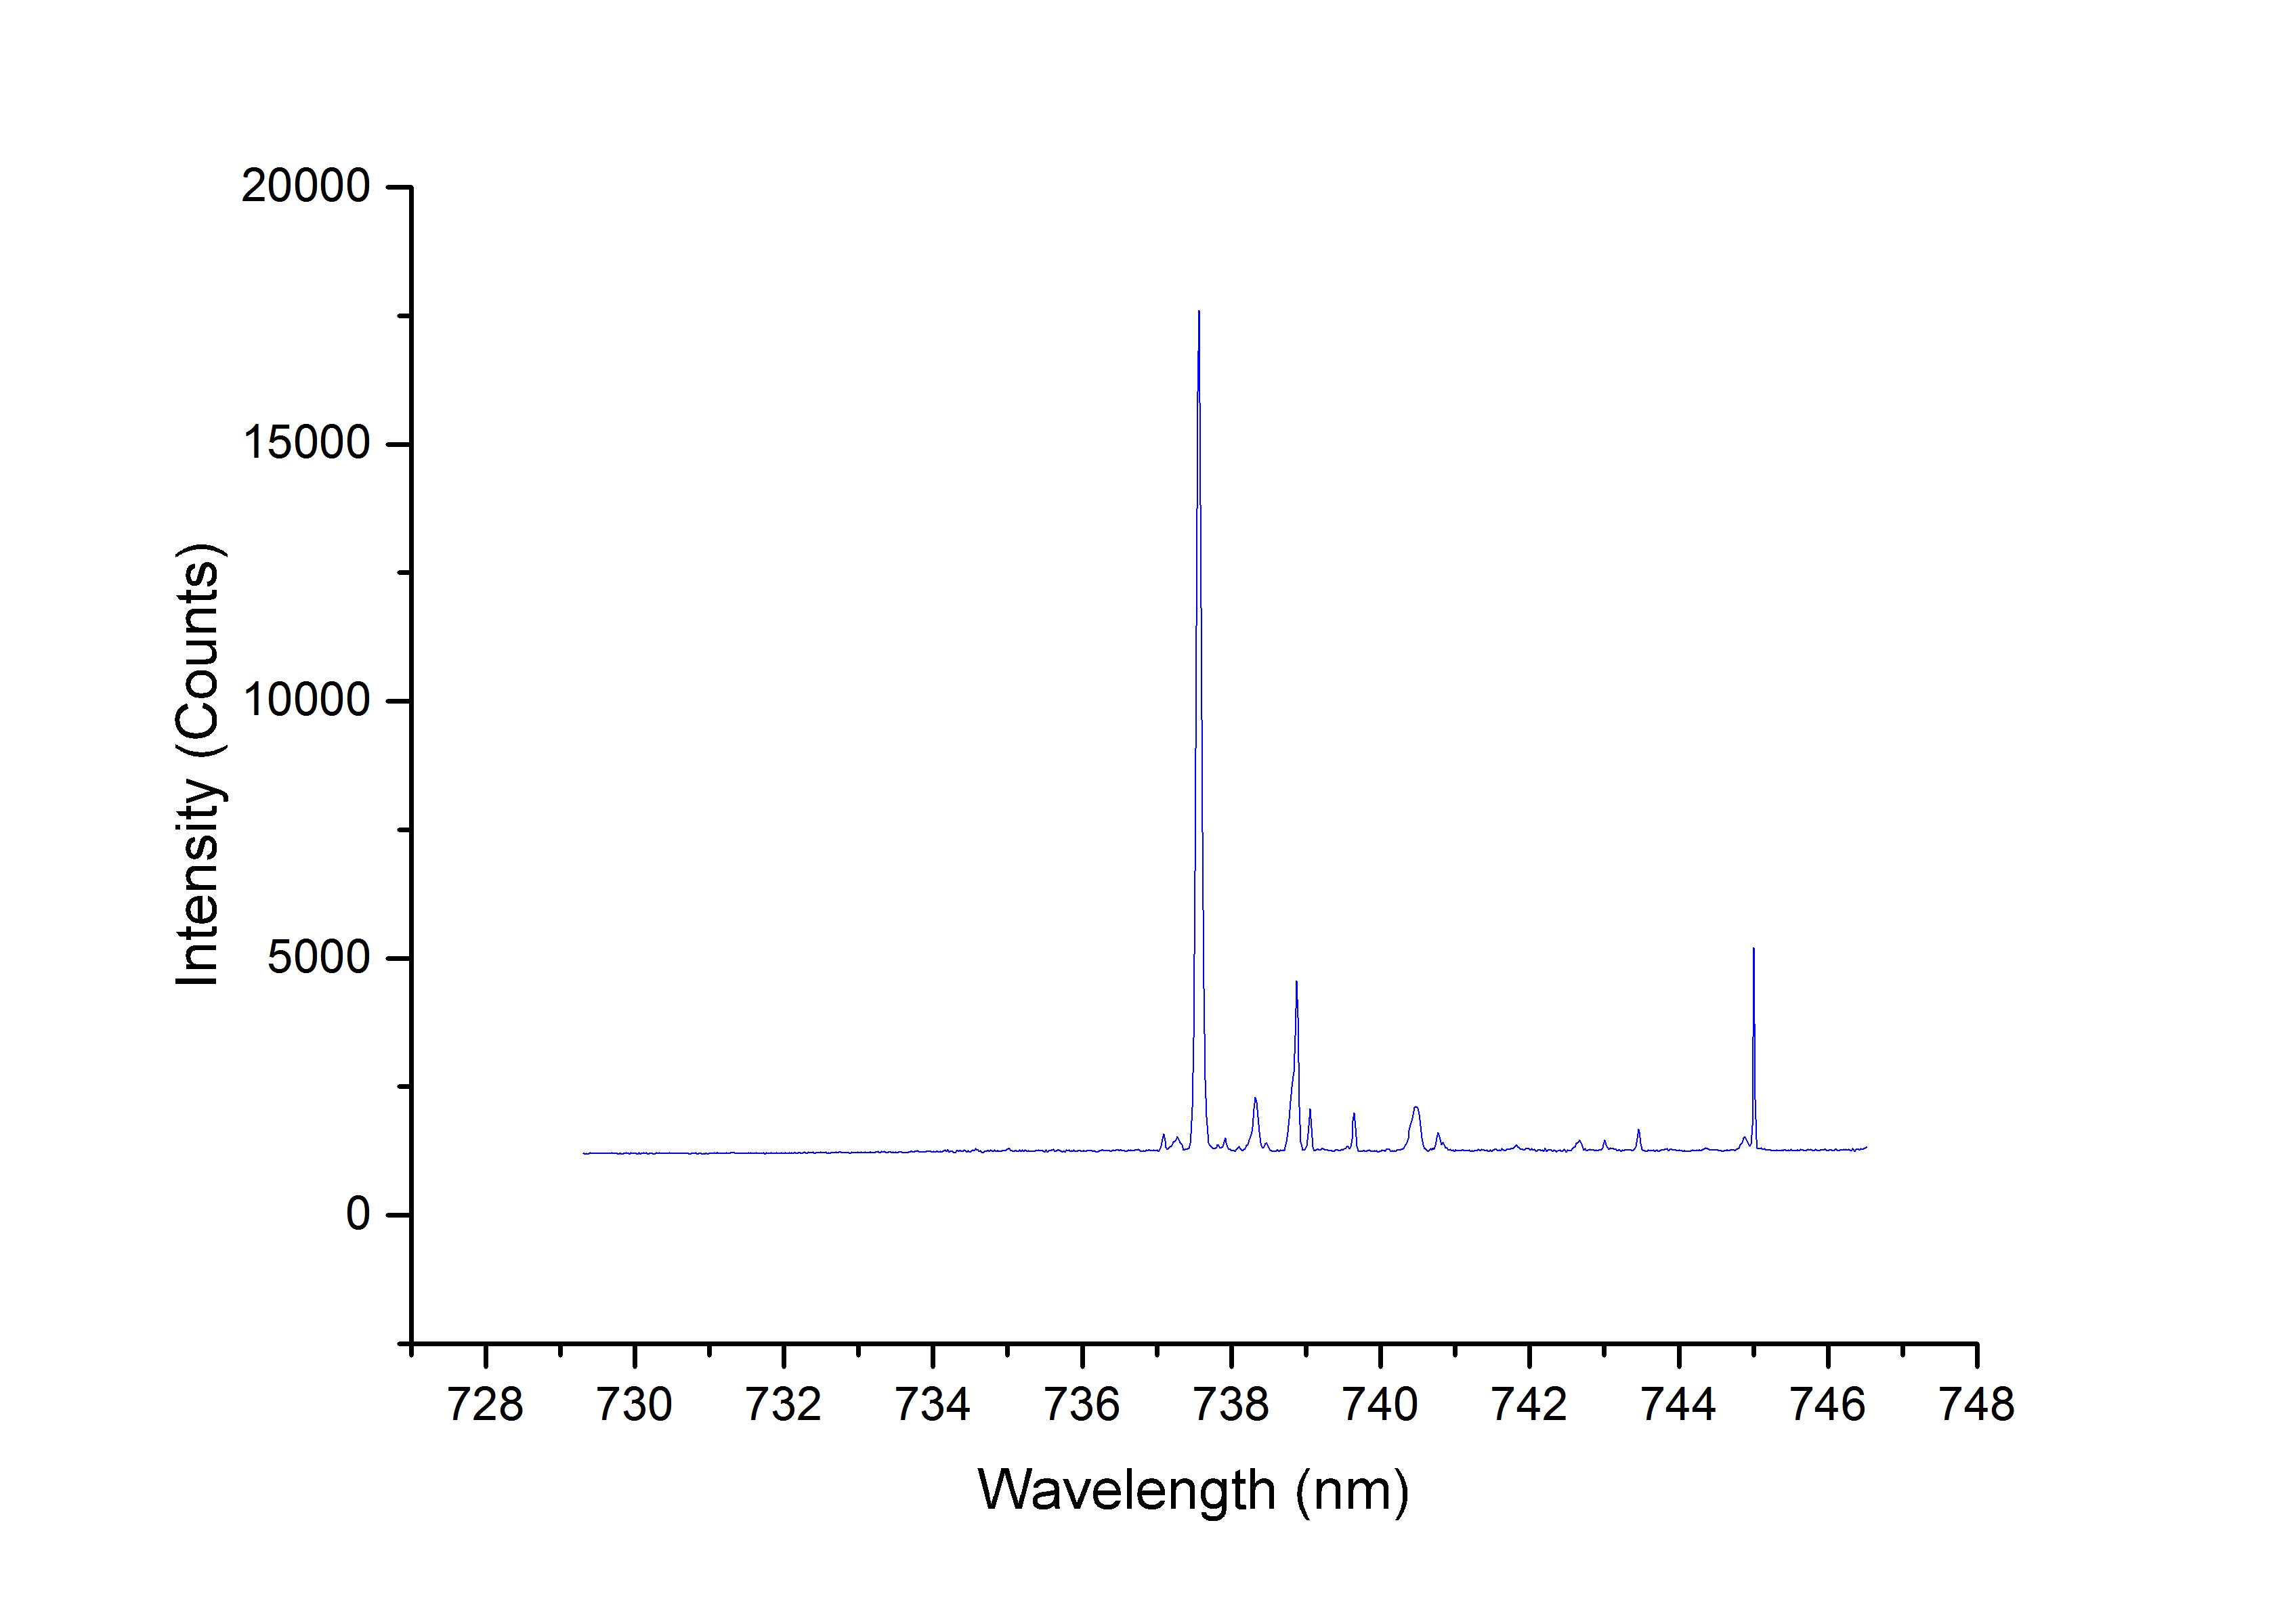
\includegraphics[trim = 0 0 0 0,  clip= true, width = \textwidth]{./pics/cryo_Spektrum84_edit.png}}
					\label{subfig::cryo2}
				\end{subfigure}
				\caption[Spectra of \nds at cryogenic temperatures]{Comparison of spectra taken at room-temperature (l.h.s) and at cryogenic temperatures (r.h.s). At low temperatures a multitude of lines is revealed indicating several \sivs embedded in a strained lattice neighborhood.}
				\label{fig::rt_vs_cryo}
			\end{figure}

			At cryogenic temperatures \psb contributions vanish, allowing a focused investigation of \zpls.
			In particular, for \sivs a four-way splitting of the \zpl is expected, see \autoref{ch::introduction}.
			To conduct low-temperature measurements, we used a confocal setup similar to the one described in \autoref{ch::pl_setup}.
			It differs merely by the fact that the sample is efficiently cooled to \SI{4}{\kelvin} using a cryostat.
			\\
			In \autoref{fig::rt_vs_cryo} measurements of two individual \nds are shown, both situated on sample \insituSo.
			\autoref{subfig::cryo1} and \autoref{subfig::cryo2} show spectra recorded at cryogenic temperatures while \autoref{subfig::roomtep1} and \autoref{subfig::roomtep2} show spectra recorded at room temperature for comparison.
			Instead of the four-fold degeneracy expected for \sivs in low-strain diamond, the cryogenic measurements indicate a multitude of various lines.
			The observation is best explained by the presence of several \sivs which are subject to varying levels of strain in their local lattice neighborhood.
			Given the fact that \zpls are found spread over a significant range of \wls, a non-negligible impact of lattice strain on \siv luminescence is revealed.
